% Report.tex
\documentclass{article}
\usepackage[utf8]{inputenc}
\usepackage{graphicx}
\usepackage{geometry}
\usepackage{float}
\usepackage{listings}
\usepackage{xcolor}
\usepackage{amsmath}
\usepackage{tikz}
\usetikzlibrary{positioning}

\geometry{a4paper, margin=1in}

\title{NA HW2 Report}
\author{Bince Qu 屈彬策 3220105862}
\date{\today}

\begin{document}

\maketitle

\tableofcontents

\section{Introduction}

This report documents the implementation of several interpolation and curve fitting tasks using reusable classes in C++. The focus is on the design of the classes, their functionalities, and the algorithms used for computations. The tasks include:

\begin{itemize}
    \item[A.] Newton Interpolation
    \item[B.] Runge's Phenomenon and Equally Spaced Nodes
    \item[C.] Runge's Phenomenon and Chebyshev Nodes
    \item[D.] Hermite Interpolation for Car Motion Prediction
    \item[E.] Newton Interpolation for Larvae Growth Prediction
    \item[F.] Curve Fitting of a Heart-Shaped Curve using Cubic Bézier Curves
\end{itemize}

\section{Class Design}

The implementation involves three primary reusable classes:

\begin{itemize}
    \item \textbf{Polynomial}: Represents a polynomial and supports various operations.
    \item \textbf{InterpCondition}: Holds interpolation conditions such as data points and derivatives.
    \item \textbf{Interp}: Performs interpolation using the Newton divided differences method or Hermite interpolation.
\end{itemize}

\subsection{Class Structure and Functionality}

The following class diagram illustrates the relationships and key components of these classes.


\begin{figure}[H]
\centering
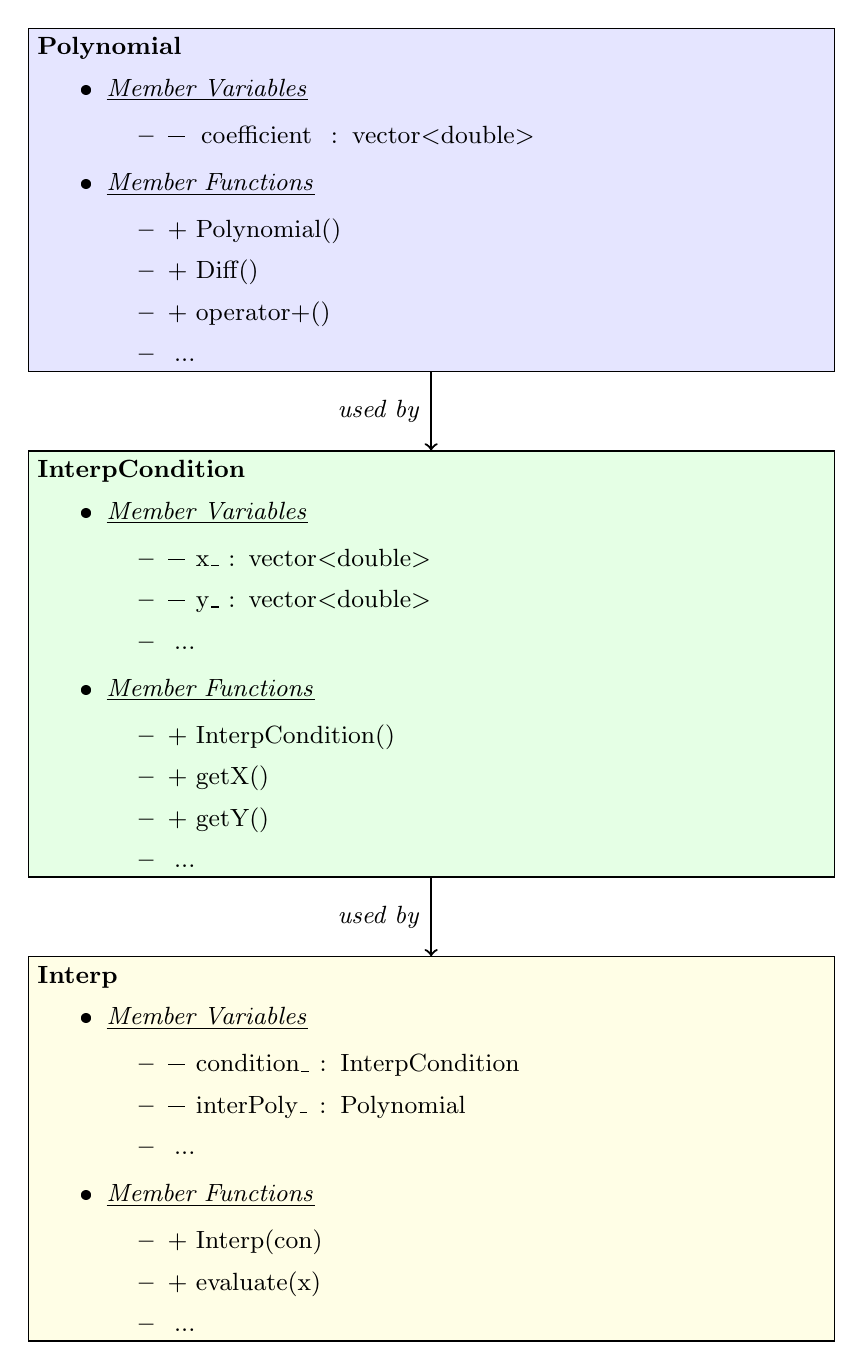
\begin{tikzpicture}[node distance=1.0cm, auto, font=\small]
    % Polynomial Class
    \node (poly) [rectangle, draw, fill=blue!10, text width=10cm] {
        \textbf{Polynomial}
        \begin{itemize}
            \item \underline{\textit{Member Variables}}
            \begin{itemize}
                \item \lstinline|- coefficient : vector<double>|
            \end{itemize}
            \item \underline{\textit{Member Functions}}
            \begin{itemize}
                \item \lstinline|+ Polynomial()|
                \item \lstinline|+ Diff()|
                \item \lstinline|+ operator+()|
                \item \lstinline|...|
            \end{itemize}
        \end{itemize}
    };

    % InterpCondition Class
    \node (interpcond) [rectangle, draw, fill=green!10, text width=10cm, below=of poly] {
        \textbf{InterpCondition}
        \begin{itemize}
            \item \underline{\textit{Member Variables}}
            \begin{itemize}
                \item \lstinline|- x_ : vector<double>|
                \item \lstinline|- y_ : vector<double>|
                \item \lstinline|...|
            \end{itemize}
            \item \underline{\textit{Member Functions}}
            \begin{itemize}
                \item \lstinline|+ InterpCondition()|
                \item \lstinline|+ getX()|
                \item \lstinline|+ getY()|
                \item \lstinline|...|
            \end{itemize}
        \end{itemize}
    };

    % Interp Class
    \node (interp) [rectangle, draw, fill=yellow!10, text width=10cm, below=of interpcond] {
        \textbf{Interp}
        \begin{itemize}
            \item \underline{\textit{Member Variables}}
            \begin{itemize}
                \item \lstinline|- condition_ : InterpCondition|
                \item \lstinline|- interPoly_ : Polynomial|
                \item \lstinline|...|
            \end{itemize}
            \item \underline{\textit{Member Functions}}
            \begin{itemize}
                \item \lstinline|+ Interp(con)|
                \item \lstinline|+ evaluate(x)|
                \item \lstinline|...|
            \end{itemize}
        \end{itemize}
    };

    % Arrows to show relationships
    \draw[->, thick] (poly.south) -- node[left]{\textit{used by}} (interpcond.north);
    \draw[->, thick] (interpcond.south) -- node[left]{\textit{used by}} (interp.north);

\end{tikzpicture}
\caption{Abbreviated Class Diagram of Reusable Classes}
\end{figure}
\subsubsection{Polynomial Class}

The \texttt{Polynomial} class represents a polynomial with methods for polynomial arithmetic, differentiation, and evaluation.

\paragraph{Member Variables}

\begin{itemize}
    \item \texttt{- coefficient : vector<double>}: Stores the coefficients of the polynomial in increasing order of degree.
\end{itemize}

\paragraph{Member Functions}

\begin{itemize}
    \item \texttt{+ Polynomial()}: Default constructor.
    \item \texttt{+ Polynomial(coef : vector<double>)}: Constructor with coefficients.
    \item \texttt{+ set\_coef(v : vector<double>) : void}: Sets the coefficients of the polynomial.
    \item \texttt{+ get\_coef() : vector<double>}: Returns the coefficients.
    \item \texttt{+ operator+(P : Polynomial) : Polynomial}: Overloaded addition operator.
    \item \texttt{+ operator-(P : Polynomial) : Polynomial}: Overloaded subtraction operator.
    \item \texttt{+ operator*(P : Polynomial) : Polynomial}: Overloaded multiplication operator.
    \item \texttt{+ operator*(scalar : double) : Polynomial}: Scalar multiplication.
    \item \texttt{+ Diff() : Polynomial}: Returns the derivative of the polynomial.
    \item \texttt{+ evaluate(x : double) : double}: Evaluates the polynomial at a given value of \texttt{x}.
\end{itemize}

\subsubsection{InterpCondition Class}

The \texttt{InterpCondition} class stores the interpolation data, including optional derivative information for Hermite interpolation.

\paragraph{Member Variables}

\begin{itemize}
    \item \texttt{- max\_order\_ : int}: The maximum order of derivative information available (0 for Newton, 1 for Hermite).
    \item \texttt{- x\_ : vector<double>}: The x-values of the data points.
    \item \texttt{- y\_ : vector<double>}: The y-values of the data points.
    \item \texttt{- y\_prime\_ : vector<double>}: The first derivatives at the data points (for Hermite interpolation).
\end{itemize}

\paragraph{Member Functions}

\begin{itemize}
    \item \texttt{+ InterpCondition()}: Default constructor.
    \item \texttt{+ InterpCondition(x\_vals : vector<double>, y\_vals : vector<double>)}: Constructor for Newton interpolation.
    \item \texttt{+ InterpCondition(x\_vals : vector<double>, y\_vals : vector<double>, y\_derivatives : vector<double>)}: Constructor for Hermite interpolation.
    \item \texttt{+ getX() : vector<double>}: Returns the x-values.
    \item \texttt{+ getY() : vector<double>}: Returns the y-values.
    \item \texttt{+ getYPrime() : vector<double>}: Returns the derivatives.
    \item \texttt{+ getOrder() : int}: Returns the maximum order of derivatives.
    \item \texttt{+ addPoint(x : double, y : double) : void}: Adds a data point.
    \item \texttt{+ addDerivative(x : double, y\_prime : double) : void}: Adds derivative information.
\end{itemize}

\subsubsection{Interp Class}

The \texttt{Interp} class performs interpolation using the Newton divided differences method or Hermite interpolation.

\paragraph{Member Variables}

\begin{itemize}
    \item \texttt{- condition\_ : InterpCondition}: The interpolation conditions.
    \item \texttt{- interPoly\_ : Polynomial}: The interpolation polynomial.
    \item \texttt{- tableOfDividedDiffs : vector<vector<double>>}: The table of divided differences.
    \item \texttt{- coefficients : vector<double>}: The coefficients of the interpolation polynomial.
\end{itemize}

\paragraph{Member Functions}

\begin{itemize}
    \item \texttt{+ Interp(con : InterpCondition)}: Constructor that performs the interpolation.
    \item \texttt{+ computeDividedDifferences() : void}: Computes the table of divided differences.
    \item \texttt{+ getInterpolationPolynomial() : Polynomial}: Constructs the interpolation polynomial.
    \item \texttt{+ evaluate(x : double) : double}: Evaluates the interpolation polynomial at a given value of \texttt{x}.
\end{itemize}

\section{Algorithm Design}

The main algorithms used in the implementation are:

\begin{itemize}
    \item Newton's Divided Differences Interpolation (Problems A, B, E)
    \item Runge's Phenomenon and Chebyshev Nodes (Problem C)
    \item Hermite Interpolation (Problem D)
    \item Curve Fitting using Cubic Bézier Curves (Problem F)
\end{itemize}

\subsection{Problem A: Newton Interpolation}

\textbf{Algorithm Steps}:

\begin{enumerate}
    \item Initialize the table of divided differences with the provided data points.
    \item Compute the divided differences iteratively for higher orders.
    \item Extract the coefficients of the interpolation polynomial from the table.
    \item Construct the Newton interpolation polynomial using the coefficients and basis polynomials.
\end{enumerate}

\subsection{Problem B: Runge's Phenomenon with Equally Spaced Nodes}

This problem demonstrates Runge's phenomenon by interpolating the Runge function using equally spaced nodes. The algorithm follows the Newton interpolation steps as in Problem A.

\subsection{Problem C: Runge's Phenomenon with Chebyshev Nodes}

To mitigate Runge's phenomenon, Chebyshev nodes are used. The algorithm includes:

\begin{enumerate}
    \item Generate Chebyshev nodes within the interval.
    \item Evaluate the function at these nodes.
    \item Perform Newton interpolation using the generated nodes and values.
\end{enumerate}

\subsection{Problem D: Hermite Interpolation for Car Motion Prediction}

\textbf{Algorithm Steps}:

\begin{enumerate}
    \item Duplicate nodes for points where derivatives are provided (as in Hermite interpolation).
    \item Modify the computation of divided differences to account for repeated nodes.
    \item Use the derivative information to compute the appropriate divided differences.
    \item Construct the Hermite interpolation polynomial.
\end{enumerate}

\subsection{Problem E: Newton Interpolation for Larvae Growth Prediction}

Similar to Problem A, Newton interpolation is used to predict the larvae growth with the given data points.

\subsection{Problem F: Curve Fitting Using Cubic Bézier Curves}

\textbf{Algorithm 2.74 Steps}:

\begin{enumerate}
    \item Select \( m+1 \) marker points \( p_0, p_1, \dots, p_m \) on the heart curve and compute the tangent vectors at these points.
    \item For each segment \( j = 0, \dots, m-1 \):
        \begin{itemize}
            \item Compute control points:
                \[
                \begin{cases}
                q_0 = p_j \\
                q_1 = p_j + \frac{1}{3}\gamma'(p_j) \\
                q_2 = p_{j+1} - \frac{1}{3}\gamma'(p_{j+1}) \\
                q_3 = p_{j+1}
                \end{cases}
                \]
            \item Construct the cubic Bézier curve for the segment using these control points.
        \end{itemize}
    \item Connect all cubic Bézier curves to approximate the full curve.
\end{enumerate}

\section{Results and Discussion}

\subsection{Problem A: Newton Interpolation}

The Newton interpolation was implemented using the reusable classes. The interpolated value at \( x = 2 \) was computed.

\begin{verbatim}
Interpolated value at x = 2 is -0.0336208
Actual value f(x) = 0.2
\end{verbatim}

\subsection{Problem B: Runge's Phenomenon with Equally Spaced Nodes}

Interpolations were performed with varying numbers of nodes to demonstrate Runge's phenomenon. The results are visualized in Figure \ref{fig:runge}.

\begin{figure}[H]
    \centering
    \includegraphics[width=0.8\textwidth]{runge_plot.png}
    \caption{Runge Function Interpolation with Equally Spaced Nodes}
    \label{fig:runge}
\end{figure}

\subsection{Problem C: Runge's Phenomenon with Chebyshev Nodes}

Using Chebyshev nodes improves the interpolation accuracy significantly, as shown in Figure \ref{fig:chebyshev}.

\begin{figure}[H]
    \centering
    \includegraphics[width=0.8\textwidth]{chebyshev_plot.png}
    \caption{Runge Function Interpolation with Chebyshev Nodes}
    \label{fig:chebyshev}
\end{figure}

\subsection{Problem D: Hermite Interpolation for Car Motion}

The Hermite interpolation was used to predict the position and speed of a car at \( t = 10 \) seconds.

\begin{verbatim}
At t = 10 seconds:
Predicted position s(t) = 742.503 feet
Predicted speed v(t) = 48.3817 feet/second
The car exceeds the speed limit of 81 feet/second.
\end{verbatim}

\subsection{Problem E: Newton Interpolation for Larvae Growth}

Newton interpolation was used to predict the weight of larvae samples after an additional 15 days.

\begin{verbatim}
Predicted weight for Sample 1 at day 43 is 14640.3 mg
Predicted weight for Sample 2 at day 43 is 2981.48 mg
Sample 1 larvae are predicted to survive after another 15 days.
Sample 2 larvae are predicted to survive after another 15 days.
\end{verbatim}

\subsection{Problem F: Heart Curve Approximation Using Cubic Bézier Curves}

The heart-shaped curve was approximated using cubic Bézier curves for \( m = 10, 40, 160 \). The approximations improve with increasing \( m \).

\begin{figure}[H]
    \centering
    \includegraphics[width=0.6\textwidth]{heart_plot_m10.png}
    \caption{Heart Curve Approximation with \( m = 10 \)}
\end{figure}

\begin{figure}[H]
    \centering
    \includegraphics[width=0.6\textwidth]{heart_plot_m40.png}
    \caption{Heart Curve Approximation with \( m = 40 \)}
\end{figure}

\begin{figure}[H]
    \centering
    \includegraphics[width=0.6\textwidth]{heart_plot_m160.png}
    \caption{Heart Curve Approximation with \( m = 160 \)}
\end{figure}

\section{Conclusion}

The use of reusable classes for polynomial representation and interpolation conditions greatly simplifies the implementation of various interpolation techniques. The modularity allows for easy extension and modification of the code for different tasks. The algorithms implemented showcase the importance of choosing appropriate interpolation methods and node selection for accurate approximations.

\end{document}
